The evaluation of our prototype consists of two parts: path discovery and bug finding. In path discovery, we evaluated different seed prioritization methods on several real-world binary programs, and in bug finding, a demo program which contains several bugs, as well as another benchmark based on real-world program, are leveraged to demonstrate the ability of our prototype system.

\subsection{Path Discovery}
To evaluate the path discovery ability of the seed prioritization method, we selected 8 programs which cover different input formats like executables, images, archives and network data. This evaluation was tested with one AFL node and lasted for 24 hours. The evaluation results were shown in Table~\ref{PD-8samples}. We have investigated the three distance measures mentioned before (i.e. EU, CS, and JI) as well as the original seed prioritization strategy (Order) from vanilla AFL which selects test case in the seed queue one by one.  

\begin{table}
  \caption{\label{PD-8samples}Path discovery for 8 sample programs}
  \centering
	\begin{tabular}{p{2cm}<{\centering} p{1.5cm}<{\centering} p{1.5cm}<{\centering} p{1.5cm}<{\centering} p{1.5cm}<{\centering}}
		\toprule
		Program  & Order\# & EU\# & CS\# & JI\# \\ 
		\midrule
		readelf  &    2753 & 4595 & 5314 & 5062 \\
		 djpeg   &    2802 & 3020 & 4198 & 3390 \\
		objdump  &    1755 & 2200 & 2960 & 2133 \\
		  gzip   &    1440 & 1564 & 1754 & 1588 \\
		 ffmpeg  &    5022 & 5993 & 6181 & 5801 \\
		tcpdump  &    3399 & 3673 & 4267 & 2950 \\
		capstone &    5626 & 6008 & 6066 & 5873 \\
		gif2png  &     912 &  981 & 1100 &  997 \\ 
		\bottomrule
	\end{tabular}
\end{table}

Figure~\ref{path-detail}(a) shows the normalized path discovery for these 8 programs based on the results in Table~\ref{PD-8samples}. From this figure, we can see that CS can achieve higher path coverage when comparing with other distance measures. And EU can also cover more paths than vanilla AFL but the performance is lower than CS. Compared with the other two distance measures, JI is the most unstable strategy which shows high path coverage for some benchmarks, like \texttt{readelf}, \texttt{djpeg}, but also brings performance overhead for some other benchmarks, like \texttt{tcpdump}.

An interesting point from Figure~\ref{path-detail}(a) is that, for \texttt{capstone}, the gain of CS is not as significant as the other 7 programs (improved only by 8\%). This is because, in our experiment, the input of \texttt{captone} was only plain texture file with some assembly code in it. Such kind of input is not as well formatted as other inputs like ELF, JPEG, CAP and so on. And modifying any parts of the input may have same possibility to trigger new behaviors which means each seed file in the queue will have nearly the same power to cover new code areas. This also demonstrates that our seed prioritization method will gain more performance for well-formatted inputs.

Figure~\ref{path-detail}(b) describes these four different prioritization strategies for four different samples according to the test time, where the x-axis indicates the test time in hours; while the y-axis shows the normalized path discovery of each strategy.
As shown in Figure~\ref{path-detail}(b), both CS and EU performed consistently better than orderly during all the 24 hours. Particularly, EU performed better than CS in the first several hours, and then CS outperformed EU in the following testing. While JI performed well in \texttt{readelf}, \texttt{ffmpeg} and \texttt{objdump}, but it failed to improve the performance in \texttt{tcpdump} after testing for 8 hours.

Based on this result, we can see that cosine similarity based seed prioritization strategy can touch more paths than other strategies. So we selected CS as our prioritization strategy in the following bug finding evaluation.
\begin{figure}
%  \centering
  \subfigure[Normalized ressults for these four prioritization strategies.]{
	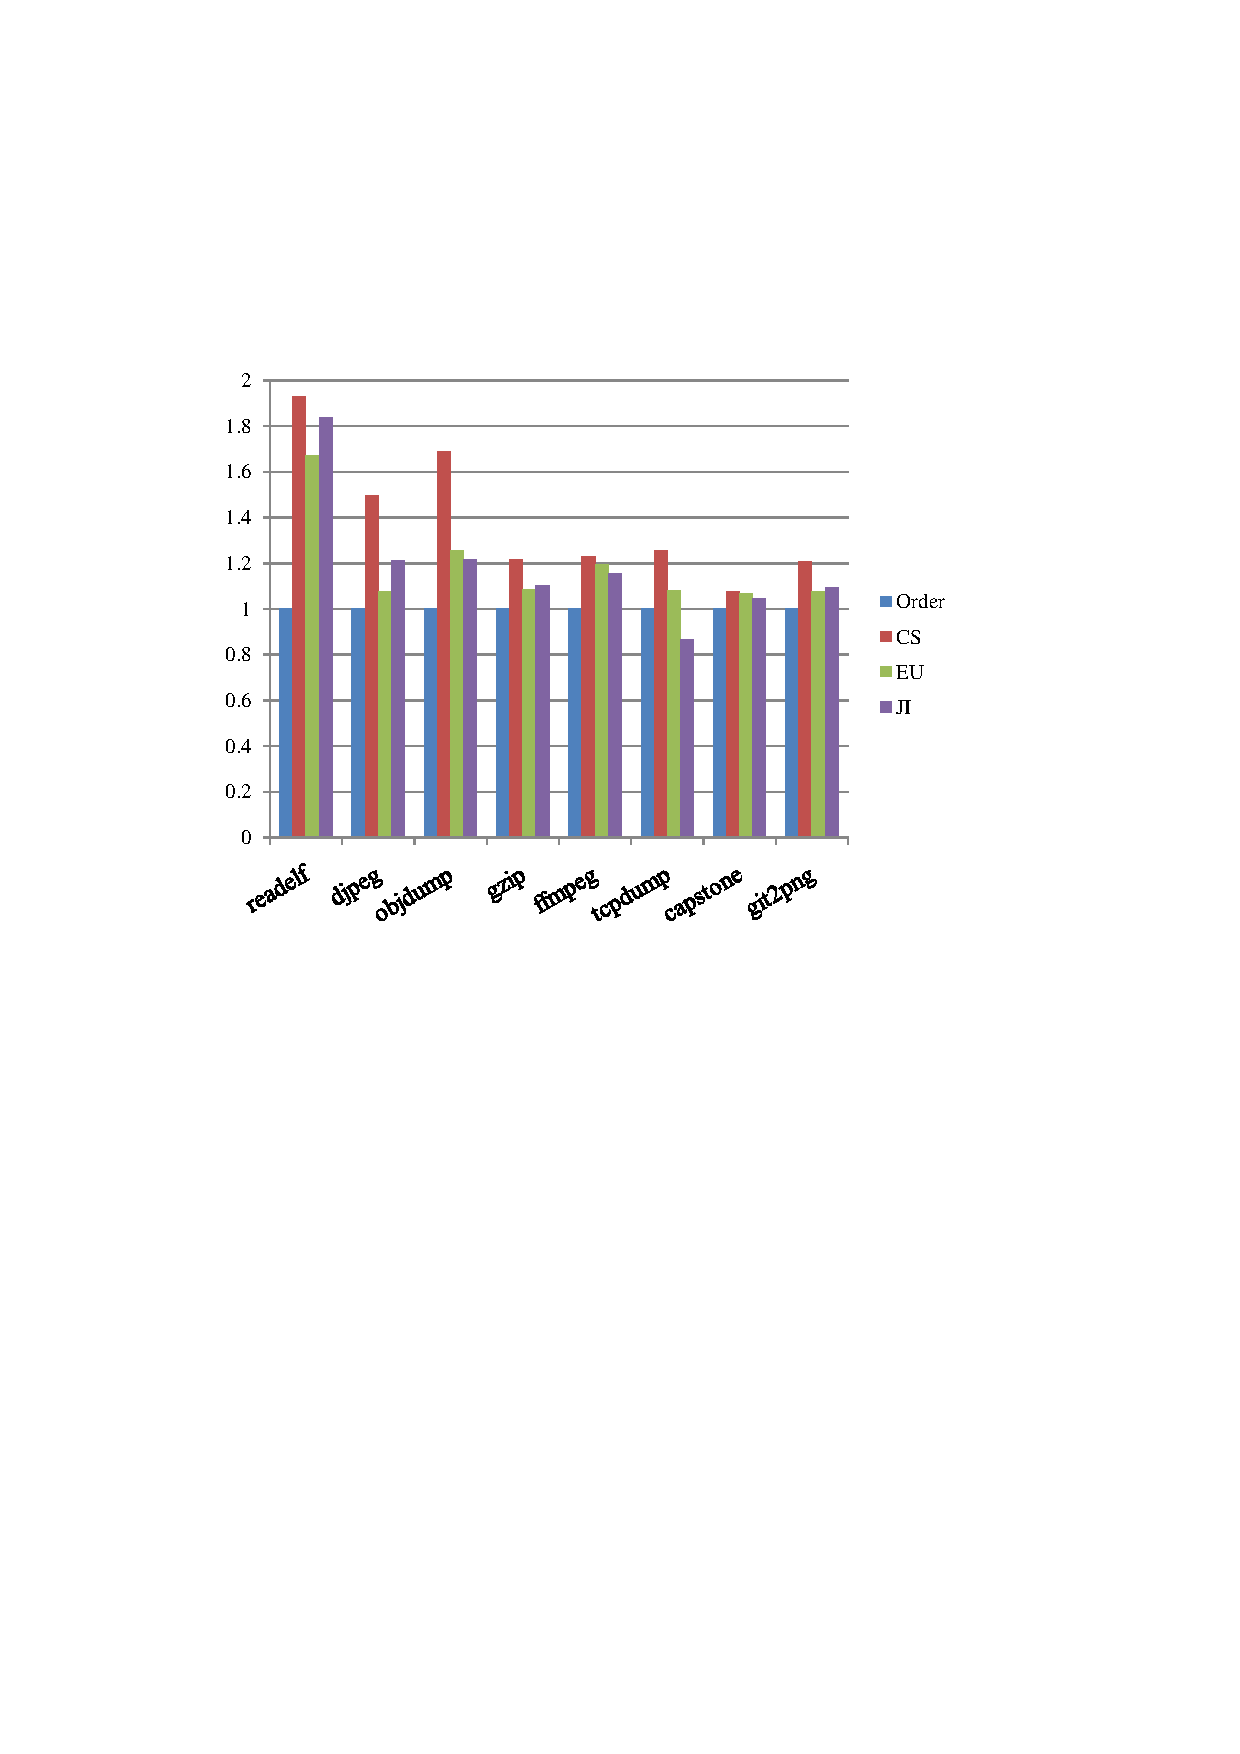
\includegraphics[width=0.5\textwidth, trim={0.4cm 0.5cm 0.3cm 0cm}, clip]{figures/path-discovery.pdf} 
  }
  \subfigure[Path discovery details along with 24 hours.]{
	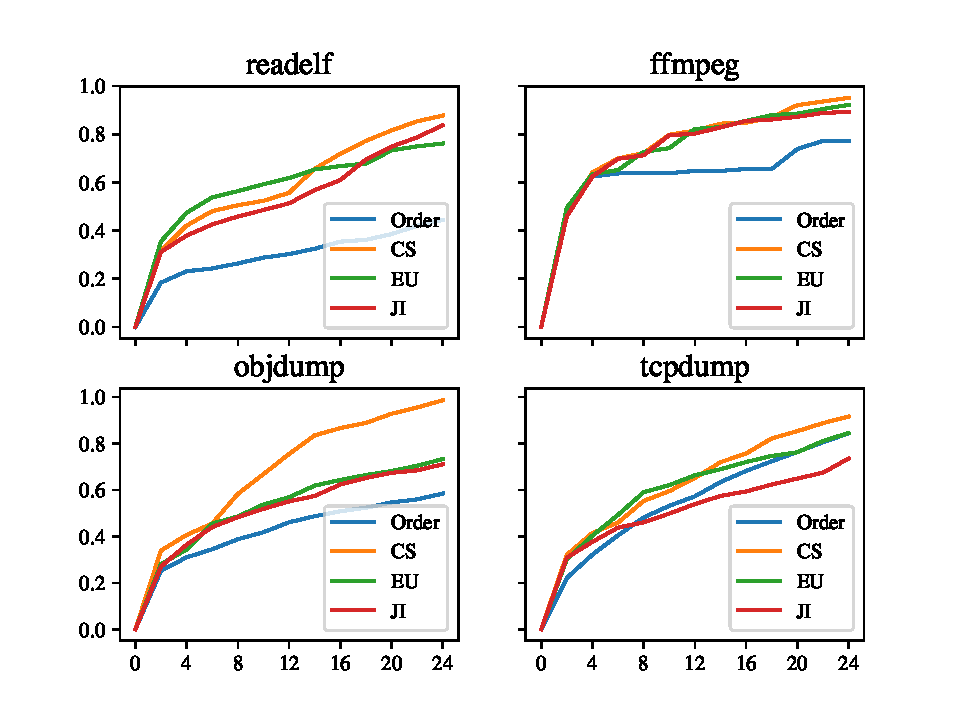
\includegraphics[width=0.48\textwidth, trim={1.3cm 0.8cm 1.5cm 0.5cm}, clip]{figures/path-time-detail.pdf} 
	}
  \caption{Path Discovery for different prioritization strategies.}
  \label{path-detail}
\end{figure} 

\subsection{Bug Finding}
We evaluated the vulnerability discovery ability of our method with two different benchmarks. The first benchmark is a demo program which is named as \emph{CommonMB}. The second benchmark is \emph{LAVA}, which is released in 2016 to test different vulnerability discovery tools \cite{dolan2016lava}. In the following sections, we are going to introduce the two benchmarks, and discuss the testing results of our prototype as well as other off-the-shelf vulnerability discovery tools (LibFuzzer \cite{libfuzzer}, AFL, KLEE, S2E, Driller, and VUzzer) in detail.

\subsubsection{CommonMB}
\noindent The \emph{CommonMB} benchmark is a demo program which contains 9 different memory error bugs. These bugs can be triggered only when feeding the program with specifically crafted input. There are four different kinds of functions in this benchmark, i.e. 2 compare-style functions, 3 math-style functions, 2 checksum-style functions and 2 logic-style functions. The compare functions contains bugs that can only be triggered when the values of specific parts of the input equal to specific constant immediate numbers; the bugs in math functions can be triggered when the results of math operation on some specific parts of the input equal to specific constant immediate numbers; the checksum related bugs can only be triggered when the input data successfully goes through the checksum checking points; and the logic bugs utilize two simple logical games (maze and semi-sudoku) as the constraints for triggering the bugs, which means the bugs can only be triggered when the testing engine successfully solves the games.

Table~\ref{CommonMB-results-detail} shows the overall results of different vulnerability discovery tools as well as our prototype with same test environment (10 cores and 12 hours).
% Explain the result like that cmp-style vulnerabiities are easy to find
We can see that all these tools have successfully triggered the two compare-style bugs (i.e. \textit{cmp16} and \textit{cmp32}). This is because there two functions are in the shallow surface of this benchmark and the conditions to trigger the bugs are simpler than the others.  

% Explain the result, for example, why add32 cannot be found by KLEE...
Fuzz testing tools discovered few bugs than symbolic execution tools in average. For example, AFL discovered the \textit{add16} and LibFuzzer triggered one more bug (i.e. \textit{add32}). But these two fuzzer both failed to uncover the bug that guarded by complex mathematic operations. All tools that leverage symbolic execution except KLEE successfully triggered all these three bugs as symbolic execution is good at solving such corner cases. One interesting point in this table is that KLEE failed to trigger \textit{add32} and \textit{complex} bugs. This is because KLEE forks too many states in checksum functions which raise the serious ``state explosion'' problem. 
% Explain why S2E can find the crc16 and crc32 but cannot find maze, this is because we maximum the coverage by rearrange the seed file?
S2E provides function models for basic functions that may fork too many states, like \textit{strcpy}, \textit{strcat}, \textit{crc16}, and \textit{crc32}. Based on these models, S2E and our prototype discovered the two bugs that related to checksum successfully. 

Logic-style vulnerabilities are difficult for all tools to uncover because the number of states will be infinite in some worse case. For example, when solving a maze, the possible oscillation between two opposite steps (such as step forward and step backward) will stop the engine from finding new paths. With the help of our seed prioritization method, our prototype successfully discovered the bug in \textit{maze} by selecting the most promising seed file to mutate.
% Explain why the sudodu is so hard to touch
However, our prototype failed to trigger the bug in \textit{sudoku}. This is because different seed files of the \textit{sudoku} have no significant differences (i.e. no more path and memory coverage), which confuses our seed prioritization method.



%Table~\ref{Prototype-result-CommonMB} shows the bug finding evaluation results of our prototype on \textit{CommonMB} benchmark. The first column lists the number of cores for the concolic execution engine, and we have tested from one core to 10 cores and collected the discovery time for each bug. 

\begin{table}
  \caption{\label{CommonMB-results-detail}Evaluation results on \textit{CommonMB} in detail}
  \centering
	\begin{tabular}{p{1.5cm}<{\centering} | p{0.8cm}<{\centering} p{0.9cm}<{\centering} | p{0.7cm}<{\centering}
	p{0.7cm}<{\centering} p{1.2cm}<{\centering} | p{0.8cm}<{\centering} p{0.8cm}<{\centering} | p{0.8cm}<{\centering} p{1cm}<{\centering} | p{1.2cm}<{\centering}}
		\toprule
	& \multicolumn{2}{c}{CMP}  & \multicolumn{3}{c}{MATH} & \multicolumn{2}{c}{CHECKSUM} & 	\multicolumn{2}{c}{LOGIC} & \\ 
	    Tool & cmp16 & cmp32 & add16 & add32 & complex & crc16 & crc32 & maze & sudoku & Total(\#) \\
		\midrule
		AFL 		& Y & Y & Y & N & N & N & N & N & N & 3 \\
		LibFuzzer	& Y & Y & Y & Y & N & N & N & N & N & 4\\
		KLEE		& Y & Y & Y & N & N & N & N & N & N & 3\\
		S2E			& Y & Y & Y & Y & Y & Y & Y & N & N & 7\\
		Driller		& Y & Y & Y & Y & Y & N & N & N & N & 5\\
		Prototype	& Y & Y & Y & Y & Y & Y & Y & Y & N & 8\\
	 \bottomrule
	\end{tabular}
\end{table}

\begin{comment}
% List this time information is useless, then comment it.
\begin{table}
\centering
  \caption{\label{Prototype-result-CommonMB}Trigger time for each bug in \textit{CommonMB}  of our prototype (in \textit{second}).}
 	\begin{tabular}{p{0.5cm}<{\centering} p{1cm}<{\centering} p{1cm}<{\centering} p{1cm}<{\centering}	p{1cm}<{\centering} p{1.5cm}<{\centering}  p{1cm}<{\centering} p{1cm}<{\centering}  p{1.5cm}<{\centering} p{1.5cm}<{\centering}}
		\toprule
	    Core & cmp16 & cmp32 & add16 & add32 & complex & crc16 & crc32 & maze & sudoku \\
		\midrule
		1 	& 4.69 & 6.32 & 4.68 & 5.72 & $>1$ hour & 5.88 & 185.66 & $>1$ hour & $>1$ hour \\
		2	& 0.02 & 2.44 & 4.31 & 0.74 & $>1$ hour & 5.14 & 2.51   & $>1$ hour & $>1$ hour \\
		4	& 0.02 & 0.24 & 4.06 & 0.32 & $>1$ hour & 4.59 & 1.50   & $>1$ hour & $>1$ hour \\
		6	& 0.02 & 0.21 & 4.16 & 0.14 & 0.48 	    & 4.67 & 2.80   & $>1$ hour & $>1$ hour \\
		8	& 0.05 & 0.21 & 4.09 & 0.15 & 1.57      & 4.58 & 1.52   & $>1$ hour & $>1$ hour \\
		10	& 0.02 & 0.20 & 4.08 & 0.30 & 1.54      & 4.57 & 1.53   & 10.86     & $>1$ hour \\
	 \bottomrule
	\end{tabular}
\end{table}
\end{comment}

\subsubsection{LAVA Benchmark}
\noindent In 2016, Dolan-Gavitt et.al. developed a technique, namely LAVA, to automatically inject secure-related bugs into some Linux utilities for evaluating the bug-finding tools. These bugs are all hard-to-reach memory errors. In the paper of LAVA, the authors describe their results on the evaluation of coverage based fuzz testing, an SAT-based approach on the benchmark. The LAVA benchmark has two corpus sets, i.e. \textit{LAVA-1} and \textit{LAVA-M}.

\textit{LAVA-1} injected 69 different bugs into the \texttt{file} program in Linux CoreUtils. There are two types of buffer overflow vulnerabilities were injected, one is \emph{Range} and the other one is \emph{Knob-and-trigger (KT)}. The Range style bugs are triggered if the magic value is in some range and also check the value to determine how much to overflow. And in the KT bug, two bytes in the input are checked against a magic value to determine if the overflow will happen and another two bytes determine how much to overflow. Both the two types of bugs were designed to mirror real bug patterns which can be used to evaluate the ability of bug-finding tools. Compared \textit{LAVA-1}, which injected only one bug in the program, \textit{LAVA-M} injected more than one bug into four different programs in CoreUtils that took file input: \texttt{base64}, \texttt{md5sum}, \texttt{uniq}, and \texttt{who}, so \textit{LAVA-M} is a better benchmark to evaluate the vulnerability discovery tools that are designed to work for a long time on programs that may contain multiple bugs.

\begin{table}
  \caption{\label{LAVA-1}Evaluation results on \textit{LAVA-1}.}
  \centering
	\begin{tabular}{p{2cm}<{\centering} p{1.5cm}<{\centering} p{1.6cm}<{\centering}  p{1.6cm}<{\centering}	p{1.5cm}<{\centering} p{1.5cm}<{\centering}  p{1.5cm}<{\centering} }
		\toprule
	    Tool & $2^0$ & $2^7$  & $2^{14}$ & $2^{21}$ & $2^{28}$ & KT \\
	         & (12 bugs) & (10 bugs) & (11 bugs) & (14 bugs) & (12 bugs) & (10 bugs) \\
		\midrule
		FUZZER 		& 0 (0\%)   & 0 (0\%)    & 1 (9\%)    & 11 (79\%) & 9 (75\%)  & 2 (20\%) \\
		SES	        & 1 (8\%)   & 0 (0\%)    & 1 (9\%)    & 3 (21\%)  & 0 (0\%)   & 1 (10\%) \\
		AFL		    & 0 (0\%)   & 0 (0\%)    & 2 (18\%)   & 10 (71\%) & 9 (75\%)  & 1 (10\%) \\
		S2E			& 3 (25\%)  & 2 (20\%)   & 3 (27\%)   & 4 (27\%)  & 3 (25\%)  & 2 (20\%) \\
		Driller		& 1 (8\%)   & 2 (20\%)   & 2 (18\%)   & 12 (86\%) & 10 (73\%) & 1 (10\%) \\
		Prototype	& 10 (83\%) & 10 (100\%) & 11 (100\%) & 13 (93\%) & 11 (92\%) & 7 (70\%) \\
	 \bottomrule
	\end{tabular}
\end{table}

Table~\ref{LAVA-1} summarized the results of bug finding evaluation on \textit{LAVA-1} from LAVA paper as well as some popular off-the-shelf tools (AFL/S2E/Driller). The maximum testing time for each bug was five hours. From this table, we can see that the \textbf{FUZZER} and \textbf{SES} mentioned in the paper only found 23 bugs and 6 bugs respectively in total. AFL found fewer paths than S2E in the small ranges ($2^0$, $2^7$ and $2^{14}$) but it outperformed S2E in larger ranges. Driller leverages the advantages of both fuzz testing and symbolic execution and the results show that it can find more paths than using them separately (28 bugs were discovered in total).

While our prototype discovered 62 bugs which was much more than the FUZZER and the SES tools separately. Particularly, we triggered all the bugs in $2^7$ and $2^{14}$ ranges. And also found most of the KT bugs (70\%) which cannot be touched effectively by the FUZZER and SES tools. Meanwhile, because of the two improvements (i.e. \textit{SLB} and \textit{LSP}), our prototype can also trigger more bugs than Driller.

Table~\ref{LAVA-M} describes the evaluation results on LAVA-M of the FUZZER and SES which are mentioned in the LAVA paper. We also listed the results of VUzzer and our prototype. 

\begin{table}
  \caption{\label{LAVA-M}Evaluation results on \textit{LAVA-M}.}
  \centering
	\begin{tabular}{p{2cm}<{\centering} p{1.5cm}<{\centering} p{1.5cm}<{\centering}  p{1.5cm}<{\centering} p{1.8cm}<{\centering}  p{1.5cm}<{\centering} }
		\toprule
	    Tool & \texttt{base64} & \texttt{md5sum} & \texttt{uniq} & \texttt{who} & Total  \\
	         & (44 bugs) & (57 bugs) & (28 bugs) & (2136 bugs) &  \\
		\midrule
		FUZZER 		& 7  & 2  & 7    & 0   & 16  \\
		SES	        & 9  & 0  & 0    & 18  & 27  \\
		VUzzer		& 17 & 1* & 27   & 50  & 95 \\
		Prototype	& 37 & 29 & 28   & 203 & 297 \\
	 \bottomrule
	\end{tabular}
\end{table}

As mentioned in the paper of LAVA, SES cannot find any bugs in \texttt{uniq} and \texttt{md5sum}. And the reasons are the control flow is too unconstrained in \texttt{uniq} and SES failed to execute any code past the first instance of the hash function. Because our symbolic execution is driven by a concrete seed input, so these two problems will be eased to a large extent which led to finding more bugs. Particularly, for program \texttt{md5sum}, VUzzer can only trigger one bug because it fails to get through the first crash to parse more of any input, whereas our prototype successfully triggered 29 bugs in \texttt{md5sum}.

\subsubsection{Real World Programs}
We selected several real world programs to evaluate the ability of unknown bug discovery of our system. The input types of this dataset cover ELF binary, multi-media, image, and packet capture. In order to demonstrate the efficiency, we also compared our results with AFL and VUzzer. We ran each program under the same testing environment with one fuzzing node for 24 hours. 

Table~\ref{zero-days} shows the results of the testing. 
% Compare with AFL
From the table we can see that during 24 hours, our prototype triggered 403 unique crashes in the dataset which outperformed vanilla AFL (181 unique crashes) and VUzzer (192 unique crashes). We can also derive from this table that our method gains little for \texttt{mp3gain} and \texttt{madplay}. This is because our symbolic execution engine does not support the float number operation when handing MPEG/WAV format (for example, all the writing operation to \texttt{XMM} registers will be concretized). This concretization lost some interesting paths and made less contribution to bug finding(only 2 more bugs for \texttt{mp3gain} and 1 more bug for \texttt{madplay}). 
This also explains the phenomena that VUzzer found more bugs in \texttt{mp3gain} than our prototype. 
It is interesting that AFL detected 15 more bugs in \texttt{elfparser} than VUzzer. This is because the fork server method leveraged in AFL enables the fuzzer can execute 51.6x more test cases than VUzzer in the same time, which can also increase the probability of finding bugs.

\begin{table}
  \caption{\label{zero-days}Zero day bugs found by our method.}
  \centering
	\begin{tabular}{l p{1.5cm}<{\centering} p{1.5cm}<{\centering} p{1.5cm}<{\centering} p{1.5cm}<{\centering} p{1.5cm}<{\centering} p{1.5cm}<{\centering} p{1.5cm}<{\centering}}
		\toprule
		& & \multicolumn{2}{c}{Prototype} & \multicolumn{2}{c}{AFL} & \multicolumn{2}{c}{VUzzer}\\
	    Program & Input & Crashes (\#) & Executed (\#)& Crashes (\#) & Executed (\#) & Crashes (\#) & Executed (\#)\\
		\midrule
		elfparser  & ELF	& 60 &   1.1M & 48   & 1.0M   & 33 & 19.0K    \\
		distorm    & ELF    & 13 &   16.2M   & 0   & 15.7M    & 3 & 93.1K    \\
		mp3gain*   & MPEG	& 43 &   11.3M  & 41  &  11.7M   & 46 &  79.3K  \\
		madplay*   & WAV	& 55 &   15.9M  & 54  & 14.3M    & 52 & 88.7K   \\
		optipng    & PNG    & 49 &   9.5M & 15  &  10.1M   & 32 & 54.1K   \\
		tstat      & PCAP   & 183&   6.4M & 23 &  6.2M   & 26 & 48.5K   \\
		\hline
		Total      &        & 403   &  & 181 &  & 192 &\\
	 \bottomrule
	\end{tabular}
\end{table}
